\chapter{Analisi del problema}
% Analisi del problema, focalizzando in particolare gli aspetti relativi alla
% concorrenza.
\section{Descrizione del problema}
Lo scopo dell'assignment è realizzare un programma concorrente che, data una directory \textit{D} presente sul file system locale contenente un insieme di documenti in PDF, provveda a determinare e visualizzare in standard output le \textit{N} parole più frequenti presenti nell’insieme dei documenti, con la rispettiva frequenza, e il numero totale di parole elaborate.\newline
Vanno ignorate (escluse dal conteggio) tutte le parole elencate in un file \textit{F} di testo che viene indicato inizialmente, nel quale è presente una parola da ignorare per riga.\newline
Si presuppone che \textit{D}, \textit{N} e \textit{F} siano parametri del programma, passati da linea di comando. È poi richiesto di estendere il programma con una GUI di modo da specificare i parametri e presentare i dati attraverso l'interfaccia.
\newline \newline
La soluzione dovrà adottare un approccio basato su programmazione multi-threaded, adottando, da un lato, principi e metodi di progettazione utili per favorire modularità, incapsulamento e
proprietà relative, dall’altro una soluzione che massimizzi le performance e reattività.

\section{Passaggio alla concorrenza}
Il problema è sicuramente risolvibile utilizzando un approccio sequenziale. La natura del problema è però tale da permetterne una certa parallelizzazione. A tale scopo è importante chiedersi:
\begin{itemize}
    \item Qual è l'algoritmo generale che risolve il problema.
    \item In quali delle sue parti è possibile ricorrere a più thread o processi per massimizzare le performance.
\end{itemize}

\noindent Viene illustrato di seguito un'esemplificazione di un algoritmo in pseudocodice per risolvere il problema:

\newpage
\begin{lstlisting}[language=Python, caption="Algoritmo semplice in pseudocodice di natura sequenziale (prima versione)"]
    Map<String, Int> result = EmptyMap()<>;
    documents = load(D);
    for(d in documents){
        pages = d.getPages();
        for(p in pages){
            words = p.getWords();
            for(w in words){
                if(w is not in file F){
                    update(result, w)
                }
            }
        }
    }
    print(firstElements(result, N))
\end{lstlisting}

\noindent In questo algoritmo i documenti PDF sono stati modellati come oggetti composti da più pagine, le quali sono composte a loro volta da più parole (Figura \ref{fig:doc-pag-wor}).

\begin{figure}[h!]
	\begin{center}
		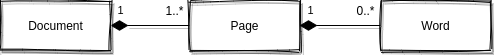
\includegraphics[width=0.85\linewidth]{img/document-page-word.png}
		\label{fig:doc-pag-wor}
		\caption{Modellazione UML di Documento, Pagina e Parola}
	\end{center}
\end{figure}

\noindent Quali sono le operazioni di questo algoritmo più dispendiose in termini di risorse? L'algoritmo prevede il caricamento in memoria dei documenti, seguito da tre cicli for annidati. La complessità del problema dipende dal numero totale dei documenti, dal numero totale di pagine e dal numero totale di parole.\newline

\noindent Per semplicità (ed anche per motivi di performance, che verranno discussi in seguito), l'algoritmo parallelo da noi scelto è uguale in tutto e per tutto alla versione sequenziale, con l'unica differenza che più documenti vengono analizzati parallelamente.
